\documentclass[10pt, compress, aspectratio=169]{beamer}

\usetheme[numbering=fraction, progressbar=none, titleformat=smallcaps]{metropolis}
\usepackage{booktabs}
\usepackage{array}
\usepackage{listings}
\usepackage{graphicx}
\usepackage[scale=2]{ccicons}
\usepackage{url}
\usepackage{relsize}
\usepackage{wasysym}

\usepackage{pgfplots}
\usepgfplotslibrary{dateplot}

\lstset{ %
  backgroundcolor={},
  basicstyle=\ttfamily\footnotesize,
  breakatwhitespace=true,
  breaklines=true,
  captionpos=n,
  commentstyle=\color{orange},
  escapeinside={\%*}{*)},
  extendedchars=true,
  frame=n,
  keywordstyle=\color{orange},
  language=bash,
  rulecolor=\color{black},
  showspaces=false,
  showstringspaces=false,
  showtabs=false,
  numbers=left,
  numbersep=3pt,
  stepnumber=1,
  stringstyle=\color{gray},
  tabsize=2,
  keywords={thrust,plus,device_vector, copy,transform,begin,end, copyin,
  copyout, acc, \_\_global\_\_, void, int, float, main, threadIdx, blockIdx,
  blockDim, if, else, malloc, NULL, cudaMalloc, cudaMemcpy, cudaSuccess,
  cudaGetLastError, cudaDeviceSynchronize, cudaFree, cudaMemcpyDeviceToHost,
  cudaMemcpyHostToDevice, const, data, independent, kernels, loop,
  fprintf, stderr, cudaGetErrorString, EXIT_FAILURE, for, dim3},
  otherkeywords={::, \#pragma, \#include, <<<,>>>, \&, \*, +, -, /, [, ], >, <}
}

\renewcommand*{\UrlFont}{\ttfamily\smaller\relax}

\graphicspath{{images/}}

\title{Uma viagem ao Kernel Linux}
\author{\footnotesize Rodrigo Siqueira \\ {\scriptsize rodrigosiqueiramelo@gmail.com} \\ {\scriptsize \url{http://siqueira.tech}} }
\institute{
\includegraphics[height=2cm]{tux}\\[0.2cm]}

\begin{document}

\maketitle

%------------------------------------------------------------------------------
\section{Parte 1: Viagem ao centro do Linux}

\begin{frame}{Visão geral da comunidade Kernel Linux}
  \begin{figure}
    \centering
    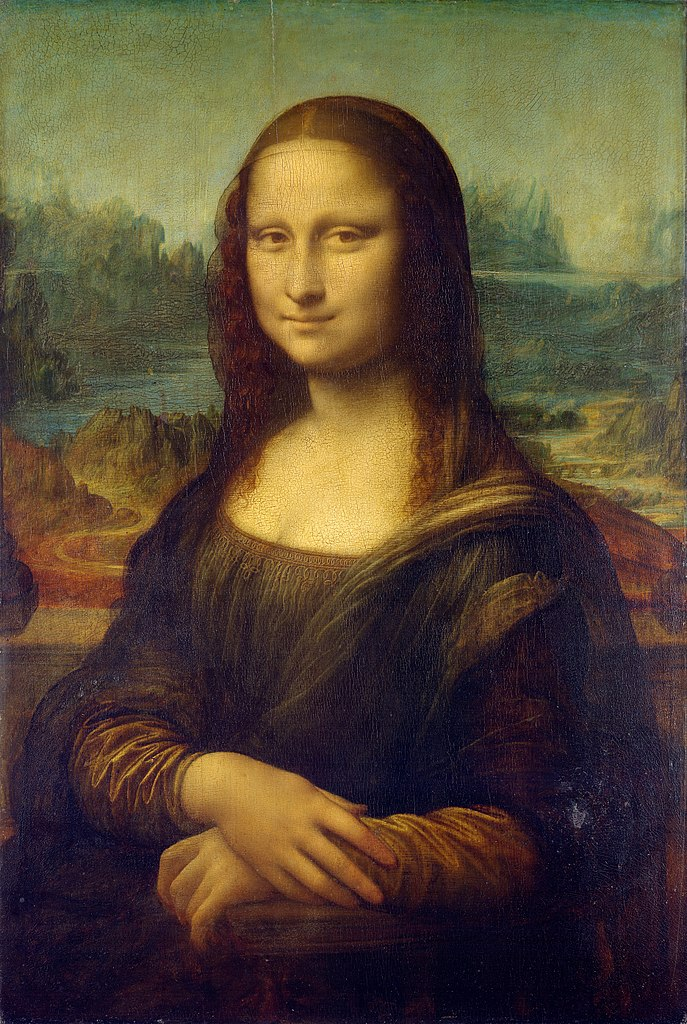
\includegraphics[width=\linewidth,
                     height=0.8\textheight,
                     keepaspectratio]{monalisa}
  \end{figure}
\end{frame}

\begin{frame}{Visão geral da comunidade Kernel Linux}
  \begin{figure}
    \centering
    
\includegraphics[width=\linewidth,
                     height=0.8\textheight,
                     keepaspectratio]{monalisa_puzzle}
  \end{figure}
\end{frame}

\begin{frame}{Alguns dos subsistemas}
  \metroset{block=fill}
  \begin{exampleblock}{Exemplos de subsistemas}
alsa-devel, autofs, backports, ceph-devel, cgroups, cpufreq, dash,
dccp, devicetree-compiler, devicetree-spec, devicetree, dmaengine,
dwarves, ecryptfs, fio, fstests, initramfs, irda-users, kernel-janitors,
kernel-packagers, kernel-testers, keyrings, kvm-commits, kvm-ia64,
kvm-ppc,   kvm,   lartc,   libzbc,   linux-8086,   linux-acpi,   linux-admin,
linux-alpha,   linux-api,   linux-apps,   linux-arch,   linux-arm-msm,
linux-assembly,   linux-bbs,   linux-bcache,   linux-block,   linux-bluetooth,
linux-btrace,   linux-btrfs,   linux-c-programming,   linux-can,   linux-cifs,
linux-clk,   linux-config,   linux-console,   linux-coverity,   linux-crypto,
linux-diald,   linux-doc,   linux-edac,   linux-efi,   linux-embedded,
linux-ext4,   linux-fbdev,   linux-fido,   linux-fpga,   linux-fscrypt,
linux-fsdevel,   linux-fsf,   linux-ftp,   linux-gcc,   linux-gpio,
linux-hams,   linux-hexagon,   linux-hotplug,   linux-hwmon,   linux-i2c,
linux-ia64,   linux-ibcs2,   linux-ide,   linux-IIO,   LInux-input,
linux-integrity,   linux-ipx,   linux-isdn,   linux-japanese,   linux-kbuild,
linux-kernel-announce,   linux-kernel-announce.posters,   linux-kernel,
linux-kselftest,   linux-laptop,   linux-leds,   linux-linuxss,
linux-lugnuts,   linux-m68k-cvscommit,   linux-m68k,   linux-man,   linux-mca,
linux-media, linux-metag,   linux-mmc,   linux-modules,   linux-msdos-devel...
  \end{exampleblock}
\end{frame}

\begin{frame}{Os Mantenedores}

 \metroset{block=fill}
  \begin{exampleblock}{Exemplos de subsistemas}
Em software livre, um mantenedor de software ou mantenedor de pacotes é
geralmente uma ou mais pessoas que criam código-fonte em um pacote binário para
distribuição, fazem commits de patches ou organizam código em um repositório.
  \end{exampleblock}

  \begin{itemize}
    \item O arquivo MAINTAINERS
    \item \texttt{scripts/get\_maintainer.pl --separator , --nokeywords --nogit --nogit-fallback --norolestats <FILE/DIR>}
  \end{itemize}
\end{frame}

\begin{frame}{Linux Foundation e Repositórios}

  \begin{figure}
    \centering
    
\includegraphics[width=\linewidth,
                     height=0.3\textheight,
                     keepaspectratio]{linux-foundation}
  \end{figure}

  \begin{itemize}
    \item \url{https://www.linuxfoundation.org/}
    \item \url{https://git.kernel.org/pub/scm/linux/kernel/git/}
    \item Algumas organizações tem seus próprios repositórios oficiais
  \end{itemize}

\end{frame}

\begin{frame}{Uma breve história do processo de desenvolvimento}

  \begin{enumerate}
    \item Escrever o código
    \item Testar o código
    \item Verificar o estilo de código
    \item Escrever uma boa menssagem de commit
    \item Encontrar os maintainers e a lista de email correta para enviar
          o patch
    \item Preparar o patch utilizando \texttt{git format-patch}
    \item Enviar o patch
    \item Esperar até 3 semanas por um feedback
    \item Ao receber um feedback, aplicar as correções e reenviar o patch
  \end{enumerate}

 \metroset{block=fill}
  \begin{exampleblock}{Links importantes: leitura obrigatória}
    \begin{itemize}
      \item Sobre o processo de desenvolvimento: \url{https://www.kernel.org/doc/html/v4.15/process/2.Process.html}
      \item Sobre o primeiro patch: \url{https://kernelnewbies.org/FirstKernelPatch}
    \end{itemize}
  \end{exampleblock}

\end{frame}

\begin{frame}{O estilo de código}

 \metroset{block=fill}
  \begin{exampleblock}{Importantes}
    \begin{itemize}
      \item \url{https://www.kernel.org/doc/html/v4.10/process/coding-style.html}
      \item \texttt{perl scripts/checkpatch.pl --terse --no-tree --color=always --codespell -strict --file <FILE>}
    \end{itemize}
  \end{exampleblock}

\end{frame}

\begin{frame}{Emails}

  Passo 1: Configurar o neomutt
  \begin{itemize}
    \item Tutorial sobre mutt: \url{http://stevelosh.com/blog/2012/10/the-homely-mutt/}
    \begin{itemize}
      \item Leia este tutorial para ter noções básicas da configuração, não se apegue aos detalhes
      \item Recomendo pular toda parte de configuração offlineimapp
    \end{itemize}
    \item Arquivo para o mutt pré-prontos: \url{https://github.com/rodrigosiqueira/myConfigFiles/tree/master/roles/neomutt/files/mutt}
  \end{itemize}

  Passo 2: Se inscrevendo em uma lista e criando filtros
  \begin{itemize}
    \item Utilizar uma conta gmail por questões de facilidade
    \item Criar um labels especificas (e.g., linux-kernel, dri-devel, etc)
    \item Configurar um filtro para redirecionar emails da lista para o label especifico
  \end{itemize}

\end{frame}

\begin{frame}{Emails: Exemplo de configuração de filtro}
  \begin{columns}[T]
    \begin{column}{.4\textwidth}
      \begin{figure}
        \centering
        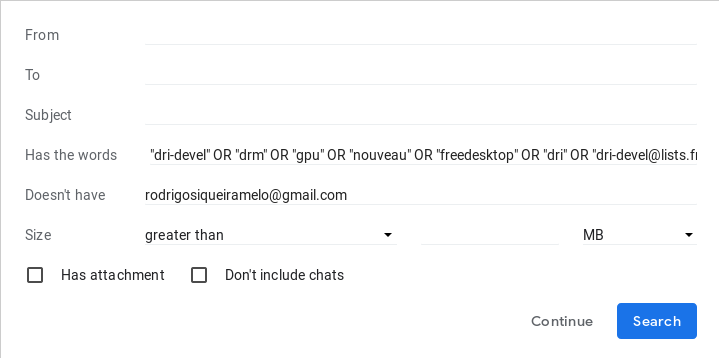
\includegraphics[width=\linewidth,
                       height=0.7\textheight,
                       keepaspectratio]{conf_filter_1}
      \end{figure}
    \end{column}

    \hfill
    \begin{column}{.5\textwidth}
      \begin{figure}
        \centering
        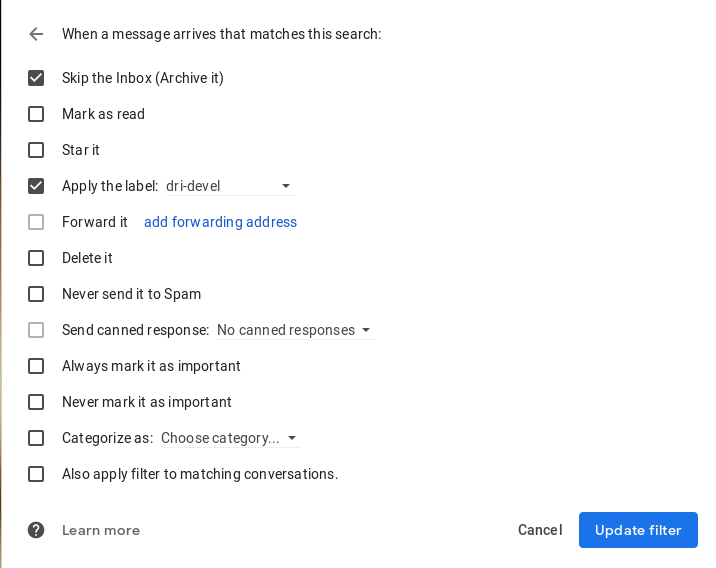
\includegraphics[width=\linewidth,
                         height=0.6\textheight,
                         keepaspectratio]{conf_filter_2}
      \end{figure}
   \end{column}
  \end{columns}

\end{frame}

\begin{frame}{IRC}
  \begin{itemize}
    \item A forma mais rápida de obter feedback da comunidade
    \item Cada subsistema tem a sua particularidade, logo, alguns estão no IRC
          e outros não
  \end{itemize}
\end{frame}

%------------------------------------------------------------------------------
\begin{frame}{O Kernel Linux}

  Compilar o Kernel, por qual motivo você faria isto? \pause

  \begin{itemize}
    \item Utilizando repositórios oficiais
    \item \texttt{git clone git://git.kernel.org/pub/scm/linux/kernel/git/torvalds/linux.git}
  \end{itemize}

\end{frame}

\begin{frame}{Uma visão geral dos arquivos}

  \begin{columns}[T]
    \begin{column}{.4\textwidth}
      \begin{itemize}
        \item arch
        \item Documentation
        \item drivers
        \item fs
        \item include
        \item init
        \item ipc
        \item Kbuild
      \end{itemize}
    \end{column}

    \hfill
    \begin{column}{.5\textwidth}
      \begin{itemize}
        \item Kconfig
        \item kernel
        \item lib
        \item LICENSES
        \item MAINTAINERS
        \item Makefile
        \item mm
        \item net
        \item README
        \item scripts
        \item tools
      \end{itemize}
   \end{column}
  \end{columns}

\end{frame}

\begin{frame}{O todo poderoso \texttt{.config}}

 \metroset{block=fill}
 \begin{exampleblock}{O que é o \texttt{.config}}
  É o arquivo que diz o que será compilado
 \end{exampleblock}

  \begin{itemize}
    \item Como obter um \texttt{.config} "funcional":
      \begin{enumerate}
        \item \texttt{zcat /proc/config.gz > .config}
        \item \texttt{cp /boot/config-`uname -r` .config}
      \end{enumerate}
    \item Uma forma de reduzir a quantidade de arquivos compilados: \newline
      \texttt{make localmodconfig}
    \item Navengando no menu de configurações \newline
      \texttt{make nconfig}
  \end{itemize}
\end{frame}

\begin{frame}{Finalmente... compilando o Kernel}
  \texttt{make -j16 \&\& make modules}
\end{frame}

\begin{frame}{Instalando}
  ATENÇÃO: Os passos aqui descritos podem variar em cada distro
  \begin{itemize}
    \item \texttt{sudo make modules\_install}
    \item \texttt{sudo make install}
    \item \texttt{sudo grub-mkconfig -o /boot/grub/grub.cfg}
  \end{itemize}
\end{frame}

%------------------------------------------------------------------------------
\section{Parte 2: Navegando no Kernel Linux com kworkflow}

\begin{frame}{O que o kworkflow?}
 \metroset{block=fill}
 \begin{exampleblock}{kworkflow (kw)}
  É um conjunto de scripts agrupados que tem por objetivo facilitar o
  ciclo de desenvolvimento no kernel Linux
 \end{exampleblock}
  \begin{itemize}
    \item Kworkflow ou kw
    \item Simples de instalar
  \end{itemize}
\end{frame}

\begin{frame}{Visão geral do kw}
  \begin{itemize}
    \item Instação: ./setup.sh -i \pause
    \item Maintainers: kw maintainers <FILE/DIR> \pause
    \item Code style: kw codestyle <FILE/DIR> \pause
    \item Preparar vm: kw prepare \pause
    \item Compilar: kw build \pause
    \item Instalar módulos: kw install \pause
    \item Compilar e instalar: kw bi
  \end{itemize}
\end{frame}

\begin{frame}{Ajuda}
  \begin{figure}
    \centering
    
\includegraphics[width=\linewidth,
                     height=0.8\textheight,
                     keepaspectratio]{want_you}
    \caption{\url{https://github.com/rodrigosiqueira/kworkflow.git}}
  \end{figure}
\end{frame}

%------------------------------------------------------------------------------
\section{Parte 3: Navegando no em você mesmo}

\begin{frame}{Boa parte do trabalho parte de você}
  \begin{figure}
    \centering
    
\includegraphics[width=\linewidth,
                     height=0.8\textheight,
                     keepaspectratio]{self_made2}
  \end{figure}
\end{frame}

\begin{frame}{Você não está sozinho...}
  \begin{figure}
    \centering
    
\includegraphics[width=\linewidth,
                     height=0.8\textheight,
                     keepaspectratio]{together}
  \end{figure}
\end{frame}

\maketitle

\end{document}
